% Chapter 4 can be included from a larger thesis with \input or \include.
% This chapter uses only citation keys already present in references.bib.
% No Chapter 4 reference entries were added to references.bib.

\chapter{Offline Data Preparation and Catalogue Construction}
\label{chap:offline_catalogue}

\section{Chapter Overview}
\label{sec:offline_overview}

The online Humanoid Matcher can make a reliable decision only if its candidate
motions and reference music have already been converted into consistent,
validated representations. This chapter describes that offline preparation
process. The input is the paired music and motion data provided by AIST++, in
which a dance is represented by an SMPL pose sequence and is associated with a
music recording \cite{li2021ai,loper2023smpl}. The outputs are two connected
resources: a searchable audio catalogue and a set of canonical Unitree G1
trajectories. A catalogue entry is admitted only when both resources are
available and the robot trajectory passes a kinematic preflight in MuJoCo.

The offline pipeline has four principal stages. First, source files and model
assets are identified by stable names and cryptographic hashes. Second, audio
is divided into overlapping analysis windows and encoded by learned and
hand-designed descriptors. Third, SMPL motion is analysed to locate low-velocity
key poses and is retargeted through General Motion Retargeting (GMR) to the
29-degree-of-freedom G1 model. Finally, the retargeted trajectory is validated,
and the resulting descriptors, motion profiles, provenance records, and dense
arrays are written as a versioned catalogue.

\section{Source Data and Reproducibility Contracts}
\label{sec:offline_sources}

\subsection{AIST++ pairing and source identity}
\label{subsec:aist_pairing}

AIST++ provides diverse 3D dance sequences with music and SMPL parameters,
making it suitable for building a retrieval catalogue rather than a single
genre-specific demonstration \cite{li2021ai}. The preparation program reads the
official split lists and associates each motion identifier with its SMPL motion
file and music identifier. A row is not silently admitted when one side of this
pair is missing. Instead, incomplete or invalid rows are recorded separately so
that catalogue size cannot be mistaken for successful processing coverage.

The dataset contains repeated uses and variants of the same underlying music.
Treating every file as an independent song would bias nearest-neighbour search
towards duplicated recordings. The audio preparation stage therefore groups
variants by music identifier, situation label, and a fingerprint computed from
the first six seconds of decoded audio. Within an identical group, the longest
recording is retained as the representative variant. This preserves meaningful
recording differences while removing byte-level or content-level duplication
that would otherwise inflate a track's influence.

Every generated motion artefact records the source motion identifier and the
SHA-256 digest of the source file. The prepared SMPL model, the GMR software
revision, the target model, and important solver settings are likewise part of
the generation contract. Consequently, equality of filenames is not treated as
evidence that two artefacts have the same meaning. A cached trajectory is reused
only if its provenance and schema agree with the current build request.

\subsection{Preparation of the SMPL body model}
\label{subsec:smpl_preparation}

SMPL represents the human body with a skinned surface, a 24-joint kinematic
structure, pose parameters, and shape parameters \cite{loper2023smpl}. The model
files required to interpret these parameters are licensed assets and are not
embedded in the project. A dedicated preparation step converts legacy array
objects into ordinary NumPy arrays and verifies the structural fields used by
the forward-kinematics code. In particular, the implementation checks a
$6{,}890\times3$ template mesh, a $6{,}890\times24$ skinning-weight matrix, a
$24\times6{,}890$ joint regressor, a $2\times24$ kinematic tree, and compatible
shape directions. All arrays must be finite.

Structural validation alone cannot detect every damaged or incompatible model
file. The prepared neutral model is therefore instantiated once in its rest
pose. The expected $6{,}890$ vertices and at least 24 finite joints must be
produced before the model is accepted. Files are written atomically only after
these checks succeed. This model preparation is intentionally separated from
the dataset build: licensing and one-time format conversion are deployment
concerns, whereas motion retargeting must be repeatable without manually
editing model data.

\section{Audio Catalogue Construction}
\label{sec:audio_catalogue}

\subsection{Windowing and robust signal preparation}
\label{subsec:audio_windowing}

All audio is decoded to mono at $16\,\mathrm{kHz}$. A track is divided into
six-second windows with a two-second hop. A short track is zero-padded, and the
last window is included even when the regular hop grid does not end exactly at
the track boundary. This policy provides full temporal coverage while keeping
the online query duration identical to the offline reference duration.

Before feature extraction, the median sample value is removed to suppress a DC
offset. The signal is then scaled by its 95th percentile absolute amplitude and
clipped to $[-1,1]$. If $x[n]$ denotes the decoded signal and
$q_{0.95}$ denotes the 95th percentile of
$|x[n]-\operatorname{median}(x)|$, the normalised waveform is

\begin{equation}
    \widetilde{x}[n]
    = \operatorname{clip}\!\left(
        \frac{0.8\left(x[n]-\operatorname{median}(x)\right)}
             {\max(q_{0.95},\epsilon)},-1,1
      \right).
    \label{eq:offline_robust_audio_normalisation}
\end{equation}

Percentile scaling is less sensitive than peak normalisation to one impulsive
sample. The factor $0.8$ leaves headroom before clipping. Signal RMS and dynamic
range are measured from the unnormalised signal, whereas learned and DSP
descriptors use the robustly normalised waveform. This distinction prevents
recording gain from dominating similarity while retaining loudness information
as optional diagnostic metadata.

The six-second, two-second policy creates overlapping reference segments. This
is deliberate. A music file may contain an introduction, a breakdown, and a
dense rhythmic passage that should not share one global descriptor. Segment
retrieval can first locate the locally relevant passage, after which evidence
may be aggregated at track level. The resulting catalogue counts are reported
with the final audio--motion join in Section~\ref{subsec:catalogue_join}, where
their admission status can be interpreted correctly.

\subsection{Learned music representation}
\label{subsec:learned_audio_representation}

Each window is passed through the official Discogs EffNet ONNX model. Models
trained with Discogs editorial metadata provide embeddings organised around
musically meaningful style information rather than generic acoustic events
\cite{alonso2022music}. The implementation obtains two outputs from the same
network:

\begin{enumerate}[label=(\arabic*)]
    \item a 1,280-dimensional embedding used for broad content and style
    similarity.
    \item a 400-dimensional vector of style-label activations used as an
    interpretable tag representation.
\end{enumerate}

Using one fixed model for both outputs avoids an undocumented combination of
incompatible learned spaces. The catalogue metadata records the backend name,
model filename, and model digest. The online extractor must satisfy the same
contract. A change of model weights is consequently a catalogue migration. Existing reference vectors must be
rebuilt before they can be compared with new queries.

\subsection{Rhythm, timbre, and activity descriptors}
\label{subsec:audio_dsp_features}

Learned embeddings are strong descriptors of musical content, but tempo and
rhythmic intensity need explicit treatment because they directly affect motion
speed and activity. The project therefore computes complementary DSP features
using short-time analysis with a 256-sample hop. The feature set includes tempo,
beat strength, onset density, off-beat ratio, tempo stability, spectral flux,
percussive ratio, three spectral-band energy ratios, mel-frequency cepstral
coefficients (MFCCs), and spectral contrast. This follows the general practice
of combining reusable music-analysis primitives with task-specific aggregation
\cite{bogdanov2013essentia}.

The scalar activity estimate is

\begin{equation}
    a = \operatorname{clip}_{[0,1]}\!\left(
        0.30b_s
        +0.30\min\!\left(\frac{d_o}{4},1\right)
        +0.20f_s
        +0.20r_p
    \right),
    \label{eq:audio_activity}
\end{equation}

where $b_s$ is beat strength, $d_o$ is onset density in events per second,
$f_s$ is normalised spectral flux, and $r_p$ is the percussive energy ratio.
The beat-quality estimate is

\begin{equation}
    q_b = \operatorname{clip}_{[0,1]}\!\left(
        0.40b_s + 0.35s_t
        +0.25\min\!\left(\frac{d_o}{4},1\right)
    \right),
    \label{eq:beat_quality}
\end{equation}

where $s_t$ measures tempo stability. These quantities have separate meanings.
Activity estimates how much motion energy the audio can support. Beat quality
estimates whether tempo-dependent decisions should be trusted. For example, a
noisy, onset-rich passage may have high activity but an unstable beat.

For compact comparison, the main handcrafted features are assembled into a
24-dimensional vector:

\begin{equation}
\begin{split}
    \mathbf{r} = [
        &\log_2(B/120), b_s, d_o/4, r_o, s_t, f_s, r_p,\\
        &\mathbf{e}_{\mathrm{band}}^{(3)},
        \boldsymbol{\mu}_{\mathrm{MFCC}}^{(8)},
        \boldsymbol{\mu}_{\mathrm{contrast}}^{(6)}],
\end{split}
    \label{eq:rhythm_timbre_vector}
\end{equation}

where $B$ is tempo in beats per minute, $r_o$ is the off-beat ratio, and the
superscripts indicate the number of retained components. The logarithmic tempo
term expresses octave-related tempo errors symmetrically. Estimates of 60 and
240 BPM are equally distant from 120 BPM in opposite directions. Per-track
reference tempo is the median of its valid segment estimates, which is more
robust than trusting a single window.

\subsection{Dense array storage and normalisation statistics}
\label{subsec:audio_array_storage}

The catalogue deliberately separates human-readable metadata from dense
numeric data. JSON stores segment identities, time ranges, scalar descriptors,
motion links, build configuration, and provenance. A compressed NPZ file stores
the matrices required for vectorised search. In the current build, these arrays
have dimensions

\begin{equation}
    \mathbf{E}\in\mathbb{R}^{348\times1280},\qquad
    \mathbf{R}\in\mathbb{R}^{348\times24},\qquad
    \mathbf{T}\in\mathbb{R}^{348\times400}.
    \label{eq:catalogue_array_shapes}
\end{equation}

The file also stores a mean and standard deviation for every embedding and
rhythm--timbre dimension. These statistics are computed only from the offline
reference set and are reused online. They must not be recomputed from a live
window, because doing so would make a query's representation depend on itself
and would destroy comparability across time. Zero or near-zero standard
deviations are guarded before standardisation. Style activations retain their
label-coordinate meaning and are unit-normalised online without
z-standardisation. The JSON and NPZ paths are tied together by catalogue
metadata so that a stale array file cannot be interpreted as belonging to a
newly generated index.

\section{Motion Key-Pose and Activity Analysis}
\label{sec:motion_analysis}

\subsection{Whole-body velocity signal}
\label{subsec:motion_velocity}

Key poses are useful entry candidates because a low-velocity posture generally
allows a smaller transition error than an arbitrary high-speed frame. The
implementation therefore derives a one-dimensional whole-body velocity signal
from each source motion before retargeting. When 3D joint positions are
available, this signal is the root-mean-square linear speed across joints. The
standard AIST++ representation used by the project contains SMPL rotations, so
the default signal is instead based on geodesic angular velocity.

Let $R_{t,j}\in SO(3)$ be the world rotation of joint $j$ at frame $t$, and let
$\Delta t$ be the frame interval. For an interior frame, the RMS angular speed
is

\begin{equation}
    v_{\mathrm{ang}}(t)=
    \sqrt{\frac{1}{J}\sum_{j=1}^{J}
    \left\|
        \frac{\operatorname{Log}\!\left(
            R_{t-1,j}^{\mathsf{T}}R_{t+1,j}
        \right)}{2\Delta t}
    \right\|_2^2},
    \label{eq:angular_velocity_signal}
\end{equation}

where $J=24$ and $\operatorname{Log}:SO(3)\rightarrow\mathbb{R}^{3}$ is the
rotation logarithm. One-sided differences are used at the endpoints. An
equivalent angular radius $r=0.35\,\mathrm{m}$ maps the result to an approximate
linear-speed scale. If root translation is present, it is first divided by the
SMPL scaling factor and combined as

\begin{equation}
    v(t)=\sqrt{\left(r v_{\mathrm{ang}}(t)\right)^2
                   +\left(w_r v_{\mathrm{root}}(t)\right)^2},
    \qquad w_r=1.
    \label{eq:combined_motion_velocity}
\end{equation}

This signal is invariant to axis--angle wrapping because it operates on
relative rotations rather than subtracting pose parameters directly. It also
prevents a dance with stationary feet but rapid upper-body motion from being
misclassified as a static sequence.

\subsection{Valley detection and key-pose confidence}
\label{subsec:keypose_detection}

The raw velocity signal is smoothed by a Gaussian kernel with a standard
deviation of $0.08$ seconds. It is then robustly mapped to $[0,1]$ using its
5th and 95th percentiles. Key-pose candidates are peaks of the negated
normalised signal, and hence valleys in body velocity. The detector enforces a
minimum temporal spacing of $0.28$ seconds, a minimum prominence of $0.08$,
and a $0.10$-second exclusion region at both sequence boundaries. These
conditions remove shallow fluctuations and avoid selecting a boundary merely
because the central-difference estimate is less reliable there.

For candidate $k$, confidence combines its peak prominence $p_k$ with its
normalised valley depth $d_k=1-\widehat{v}_k$:

\begin{equation}
    s_k=\operatorname{clip}_{[0,1]}
        \left(0.65p_k+0.35d_k\right).
    \label{eq:keypose_score}
\end{equation}

Each retained key pose stores its frame index, time, normalised clip phase,
score, prominence, and velocity. If a maximum count is requested, candidates
are first selected by confidence and are then returned in temporal order. This
avoids the common failure in which uniform temporal subsampling discards the
only strong pause in a sequence.

The detector does not claim that every velocity minimum is a musically
meaningful choreographic boundary. Instead, it constructs a set of mechanically
favourable entry hypotheses. During online preparation, these hypotheses are
ranked again using the current robot pose, velocity, contact state, and desired
phase. Separating offline proposal generation from online entry evaluation
keeps the live search small without fixing a transition choice prematurely.

\subsection{Motion profile and catalogue groups}
\label{subsec:motion_profile}

In addition to individual key poses, the analyser records summary statistics
that are inexpensive to compare online. They include median and 90th-percentile
velocity, clip duration, key-pose count, unweighted key-pose density, confidence-
weighted density, and interval regularity. If the intervals between successive
key poses are $\Delta\tau_i$, irregularity is measured by their coefficient of
variation,

\begin{equation}
    c_v=\frac{\operatorname{std}(\Delta\tau_i)}
              {\operatorname{mean}(\Delta\tau_i)+\epsilon}.
    \label{eq:keypose_interval_cv}
\end{equation}

Low $c_v$ indicates a more regular sequence of pauses, while high $c_v$
indicates irregular phrasing. Weighted density distinguishes a clip with many
weak numerical valleys from one with several pronounced key poses.

For catalogue organisation, motions are grouped by genre and coarse activity
attributes. Median velocity and weighted key-pose density are divided at the
dataset tertiles. Regularity is divided at its median. The present catalogue's
velocity cut points are approximately $1.10$ and $1.51\,\mathrm{m\,s^{-1}}$ on
the equivalent-speed scale, while density cut points are approximately $0.59$
and $0.85\,\mathrm{s^{-1}}$. These thresholds are derived from the catalogue. 
Their purpose is to support
stratified diversity choices and interpretable diagnostics without requiring a
learned motion-style classifier.

\section{SMPL-to-G1 Retargeting}
\label{sec:offline_retargeting}

Figure~\ref{fig:smpl_g1_same_frame} compares the source human mesh with the
stored G1 trajectory at identical frame indices. The examples are selected
from source-motion wrist separation and height, rather than from target-fit
quality. They illustrate preservation of broad gestures alongside changes in
body proportions and joint configuration; they are qualitative examples,
not evidence of dynamic tracking or contact stability.

\begin{figure}[htbp]
    \centering
    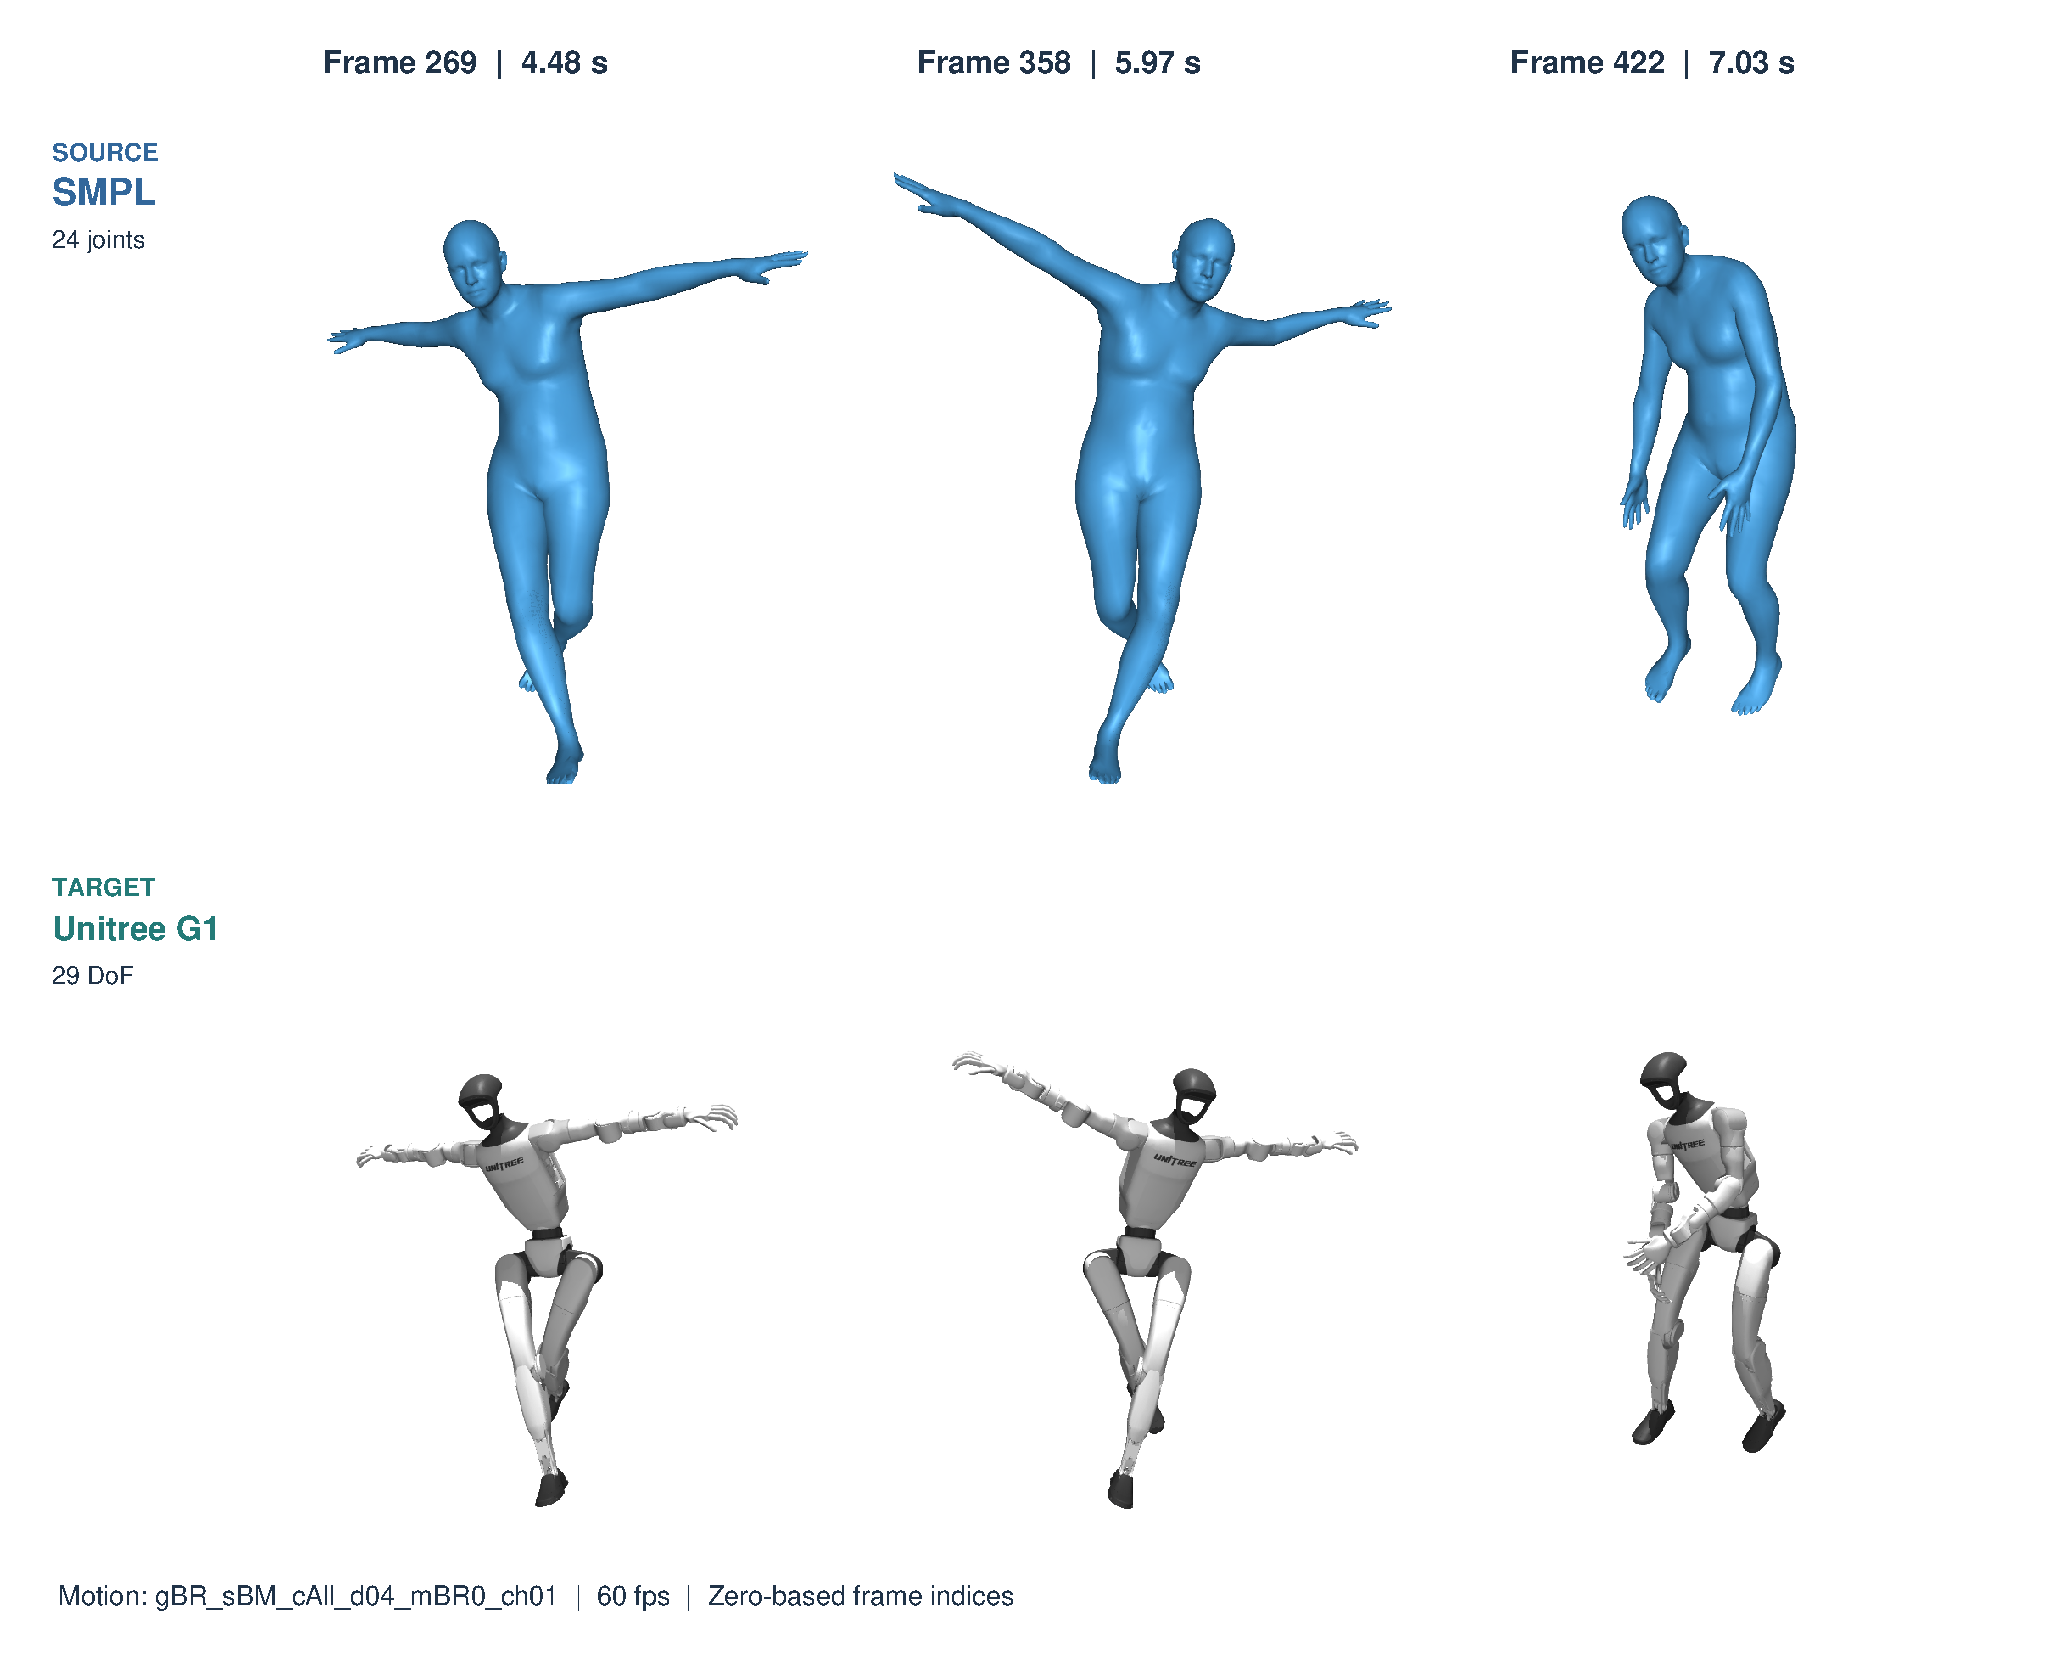
\includegraphics[width=\textwidth]{figures/chapter4_smpl_g1_same_frame.pdf}
    \caption{Same-frame SMPL-to-G1 retargeting comparison for AIST++ sequence
    \texttt{gBR\_sBM\_cAll\_d04\_mBR0\_ch01}. The neutral SMPL source mesh
    (top) and stored GMR-retargeted G1 poses (bottom) are shown at zero-based
    frames 269, 358, and 422 of the 60~fps sequence. Each column uses the same
    frame, camera, and metric scale. For display, each body is independently
    centred horizontally and grounded vertically; joint rotations are
    unchanged, so absolute root translation and ground clearance are not
    compared. Source and SMPL-model hashes were verified against the target
    artefact.}
    \label{fig:smpl_g1_same_frame}
\end{figure}

\subsection{Human forward kinematics and coordinate conversion}
\label{subsec:human_fk}

The AIST++ pose at each frame contains local axis--angle rotations for the 24
SMPL joints and, when available, root translation. Retargeting individual local
angles directly would ignore the different kinematic trees and proportions of
the human and robot. The implementation therefore composes rotations through
the complete SMPL hierarchy to obtain world-space joint positions and
orientations. Root translation is divided by the sequence's SMPL scale before
being applied.

AIST++/SMPL motion is expressed in a $Y$-up convention, whereas the target
MuJoCo model is $Z$-up. Positions and orientations are transformed by

\begin{equation}
    C_{Y\rightarrow Z}=
    \begin{bmatrix}
        1 & 0 & 0\\
        0 & 0 & -1\\
        0 & 1 & 0
    \end{bmatrix}.
    \label{eq:yup_to_zup}
\end{equation}

World rotations are converted to scalar-first quaternions
$[q_w,q_x,q_y,q_z]$. Because $\mathbf{q}$ and $-\mathbf{q}$ encode the same
rotation, quaternion signs are made temporally continuous. This apparently
small step is essential: an untreated sign flip appears as a large angular
change to interpolation and velocity calculations even though the physical
orientation is unchanged.

Fourteen human transforms are supplied as GMR targets: pelvis, upper spine,
left and right hips, knees, feet, shoulders, elbows, and wrists. This subset
captures root placement, leg contacts, torso orientation, and expressive arm
motion while leaving GMR to resolve the different source and target skeletons.
The method follows the general principle that retargeting quality materially
affects the feasibility of subsequent humanoid tracking
\cite{araujo2025retargeting}.

\subsection{GMR inverse-kinematics solve}
\label{subsec:gmr_solve}

The target is the free-root Unitree G1 model with 29 actuated joints. For every
source frame, GMR solves a constrained inverse-kinematics problem that balances
the selected human transforms against the robot kinematic structure and joint
limits. The implementation uses the DAQP-based solver with velocity limiting.
A symmetric two-step arm seed is applied before the sequence solve to reduce
the risk that the nonlinear optimiser enters a mirrored arm configuration.

Reproducibility requires control of library interfaces as well as data files.
The checked GMR revision expects an earlier positional form of the Mink
inverse-kinematics API, whereas the installed Mink version assigns a different
meaning to the corresponding argument. A narrow compatibility adapter maps the
call explicitly and records the detected limits-API mode in every artefact.
Without this adapter, the program can either fail at runtime or, more
dangerously, run with constraints in the wrong parameter position. The adapter
is kept at the integration boundary rather than modifying the optimisation
algorithm.

\subsection{Collision-aware retargeting}
\label{subsec:collision_retargeting}

Pose matching alone can place a robot hand through its torso or allow opposite
limbs to intersect. Collision avoidance is therefore enabled during trajectory
generation. The project's G1 self-collision preset defines nine groups of
non-adjacent body pairs. Adjacent links are omitted because their meshes
naturally overlap around a joint and would create persistent false constraints.
Hand geometries that are visual-only in the source model are activated for
collision evaluation.

The current preset uses a $5\,\mathrm{mm}$ minimum separation, an
$80\,\mathrm{mm}$ detection distance, a gain of $0.85$, and no constraint-bound
relaxation. Validation uses a $6\,\mathrm{mm}$ separation requirement, providing
a $1\,\mathrm{mm}$ numerical buffer beyond the generation constraint. The
expanded preset currently yields 226 geometry pairs, although this count is
recorded rather than assumed because a robot-model revision may change the
geometry set.

Collision validity is checked against both the GMR retargeting model and the
MuJoCo playback model. This dual-model check matters because different XML
files can use different meshes, contact exclusions, or visual/collision roles.
Where shallow contact behaviour differs between MuJoCo versions, the validator
uses explicit geometry-distance queries so that the intended separation
contract remains visible. The scope of this kinematic validation is stated with
the complete preflight procedure in Section~\ref{subsec:mujoco_preflight}.

\subsection{Continuity conditioning}
\label{subsec:retarget_continuity}

Even a collision-free per-frame solution can contain an abrupt change between
neighbouring frames. After retargeting, joint positions are first clamped for
minor numerical overshoot beyond their model limits. Root quaternions are
renormalised and their signs are made continuous. Segment velocities are then
limited to

\begin{equation}
    \|\dot{\mathbf{q}}_{\mathrm{joint}}\|_{\infty}
        \leq 3\pi\;\mathrm{rad\,s^{-1}},\qquad
    \|\dot{\mathbf{p}}_{\mathrm{root}}\|_2
        \leq 3\;\mathrm{m\,s^{-1}},
    \label{eq:retarget_linear_limits}
\end{equation}

and root angular speed is limited to $4\pi\,\mathrm{rad\,s^{-1}}$. For a
violating segment, the correction is not accepted solely from endpoint tests.
The candidate interpolation is sampled at 40 intermediate poses and checked
against the collision constraints. A 14-iteration binary line search finds the
largest safe progress towards the proposed frame. Two stabilisation passes are
used because restricting one segment changes the starting state of the next.
If the first retargeted frame is colliding, it is backed off towards the neutral
configuration.

This stage conditions the source trajectory but does not close its loop. A
forced last-to-first match would change valid one-shot motion and hide the real
seam that the online transition controller must handle. Loop suitability and
clip-to-clip blending are therefore addressed during playback.

\section{Canonical Trajectory and Dataset Build}
\label{sec:canonical_dataset}

\subsection{Canonical G1 artefact}
\label{subsec:canonical_artifact}

Each successfully retargeted dance is stored as a canonical binary artefact.
Its primary arrays are

\begin{equation}
    \mathbf{P}\in\mathbb{R}^{N\times3},\qquad
    \mathbf{Q}_{r}\in\mathbb{R}^{N\times4},\qquad
    \mathbf{Q}_{j}\in\mathbb{R}^{N\times29},
    \label{eq:canonical_motion_arrays}
\end{equation}

representing root position, root orientation in \texttt{wxyz} order, and G1
joint positions. The stored joint-name list fixes the semantic order of all 29
columns. Array width alone is insufficient because two 29-DoF models may use a
different order. The artefact also stores frame rate, format and pipeline
versions, source identifier and digest, SMPL-model digest, retargeter name and
full revision, collision settings, compatibility mode, and continuity limits.


\subsection{Cached builds, quarantine, and atomic publication}
\label{subsec:dataset_build_management}

Retargeting hundreds of clips is expensive, so the builder supports validated
reuse. Before reuse, a cached artefact is checked for the expected schema,
source and model hashes, complete GMR revision, frame rate, joint order,
quaternion convention, collision preset, and continuity settings. Array shapes,
finite values, quaternion norms, and sign continuity are checked as well. A
file that fails validation is renamed with an \texttt{.invalid} suffix rather
than being left under its canonical name.

New trajectories are generated to a temporary \texttt{.build} path. Only a
fully validated output atomically replaces the canonical path. Dataset
manifests follow the same publish-after-validation rule. A complete build of an
official split may replace its manifest. A partial build is merged so that an
interrupted experiment does not erase unrelated valid rows. Failed identifiers
are removed from the active manifest and written to a separate failure report.

These measures turn the manifest into a declaration of validated availability.
They also make interrupted builds recoverable. The
next run can reuse verified artefacts, quarantine incompatible ones, and
continue without assuming that an existing filename is complete.

\section{Trajectory Preflight and Catalogue Admission}
\label{sec:preflight_admission}

\subsection{MuJoCo kinematic preflight}
\label{subsec:mujoco_preflight}

The catalogue builder treats trajectory loading as a testable operation. The
preflight validator first repeats the canonical schema and provenance checks.
It rejects non-finite arrays, an unexpected joint order, invalid quaternion
norms, missing source identity, disabled collision generation, or an abbreviated
software revision. It also applies secondary corruption thresholds of
$20\,\mathrm{rad\,s^{-1}}$ for joint speed, $10\,\mathrm{m\,s^{-1}}$ for root
translation, and $20\,\mathrm{rad\,s^{-1}}$ for root angular speed. These are
looser than the generation limits in Section~\ref{subsec:retarget_continuity}.
Their role is to detect malformed data.

The trajectory is then loaded into the headless G1 playback model and grounded.
For each frame, the validator checks finite joint values and actual model joint
ranges. At a fixed stride of four frames it writes the kinematic state into
MuJoCo and calls forward evaluation. Generalised position, velocity, and
actuator-state arrays must remain finite, and the minimum foot height must not
fall below $-10^{-5}\,\mathrm{m}$ after grounding. No actuator command is
applied in this test.

Preflight is therefore a kinematic admission test. It catches schema mismatch, model-order
errors, invalid states, excessive discontinuities, and grounding failure at
catalogue-build time. Dynamic tracking, torque limits, balance, and hardware
safety require a later controller and a separate experimental evaluation.

\subsection{Joining audio and motion records}
\label{subsec:catalogue_join}

After preflight, the builder joins each valid motion profile to its music
segments. A row enters the searchable catalogue only if the audio source,
source SMPL motion, canonical G1 artefact, key-pose profile, and preflight result
are all present. Excluded rows are written to a dedicated CSV file with a
machine-readable reason. This strict inner join prevents a high-scoring audio
entry from referring to a motion that the online process cannot load.

The current catalogue contains 411 paired manifest
rows. All 411 motion rows passed admission in the recorded build, with zero
excluded motions. Because several dances share music, these rows refer to 60
music identifiers, 70 representative audio variants, and 348 audio segments.
The global median equivalent motion speed is approximately
$1.31\,\mathrm{m\,s^{-1}}$. These figures document the current artefact. A rebuild with different data, model
weights, or validation settings must update them.

\section{Integrity Guarantees and Remaining Limitations}
\label{sec:offline_integrity}

The finished offline catalogue provides five guarantees to the online matcher.
First, the query and reference audio paths share one documented extractor and
one learned-model identity, so their descriptors are compared within a
consistent feature space. Second, dense matrices have known dimensions and
reference-set normalisation statistics, preserving comparability across live
queries. Third, every selectable motion has stable source and retargeting
provenance, including source and model hashes, software revision, and generation
settings. Fourth, key poses and activity statistics have been computed
consistently from the source sequence, providing comparable entry candidates
and motion profiles. Fifth, the exact trajectory can be loaded, grounded, and
evaluated in the target MuJoCo kinematic model, with its joint ordering,
numerical validity, and model compatibility checked before admission.

Together, these guarantees establish a traceable connection between an audio
retrieval result and an available robot trajectory. Validated caching,
quarantine of incompatible artefacts, and atomic publication reduce the risk
of exposing stale or incomplete outputs. The final audio--motion join further
ensures that searchable entries refer to motions with the required profiles
and preflight results. These guarantees remain specific to the recorded data,
model assets, and validation settings. Changes to those dependencies require
the corresponding artefacts to be rebuilt or revalidated.

But these guarantees stop short of several stronger claims. A
Discogs-derived embedding is not a direct measure of choreographic correctness:
musical similarity does not establish that a particular motion suits the
phrasing or expressive intent of a new passage. A velocity valley is not
necessarily a semantic dance boundary, and a low-velocity source pose does not
by itself guarantee a smooth transition from the robot's current state.
Retargeting and continuity conditioning may also alter the motion around a
source-derived key pose, so entry suitability still requires online evaluation.

IK and self-collision constraints do not prove balance, torque feasibility, or
safe hardware execution. The MuJoCo preflight evaluates kinematic states
without applying actuator commands, and its sampled checks do not establish
continuous-time dynamic feasibility. Likewise, validating individual clips
does not validate every possible blend, loop seam, or playback-speed change.
Finally, AIST++ pairings reflect the choreography in the dataset and may not
cover arbitrary live music or all desired G1 behaviours.


